\documentclass[11pt]{rapport-tp-qlm}
% Pour les documents écrits en général, entre 10pt et 12pt
% 11pt OBLIGATOIRE POUR LE RAPPORT de l'UE Devenir Étudiant.e

% Bonne lecture des lettres accentuées :
\usepackage[utf8]{inputenc}
% si ça ne marche pas sur des systèmes un peu anciens, à la place
% de [utf8] on peut essayer [cp1252] sur Windows, ou [latin1] sur
% Mac ou Linux / Ubuntu / Fedora

% Choix d'une police de caractères :
\usepackage{lmodern}
% Dizaines d'autres possibilités, par exemple iwona, charter... 
% Voir par exemple  http://www.tug.dk/FontCatalogue/mathfonts.html
\usepackage[T1]{fontenc} % Nécessaire avec certaines police
\usepackage[section]{placeins}
% Les paquets suivants permettent d'inclure des liens internets,
% des images, des pages pdf :
\usepackage{hyperref}
\usepackage{graphicx}
\usepackage{pdfpages}
\usepackage{listings}
\usepackage{float}
\usepackage{graphicx}
\graphicspath{ {./assets/} }
%%%%%%%  FIN DE L'EN-TÊTE - DÉBUT DU CONTENU %%%%%%
\begin{document}


\title{Rapport TP 3 - IFT3913}

\author{
	\\Loïc Daudé Mondet
	\\20243814 -- Programmes d'échanges - 1er c.(Échange)
	\\
	\\Alaa edlin Yacoub
}

\date{18/11/2022}

\maketitle

\chapter{Boîtes à moustache et distribution des données}
    \section{NOCom}
    \begin{figure}[h]
    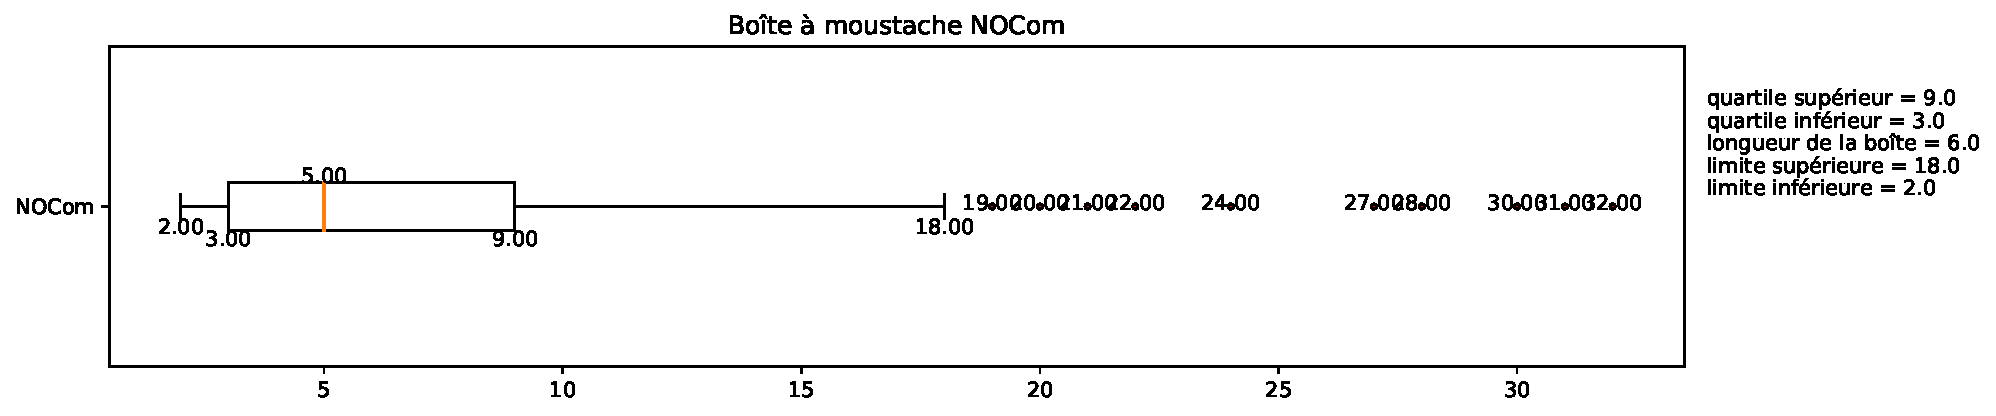
\includegraphics[scale=0.5]{assets/moustache_NOCom}
    \centering
    \end{figure}
    La boîte n'est pas symétrique ce qui signifie que les variables ne sont pas normalement distribuées, conclusion renforcée par le grand nombre de valeurs extrêmes.
    \section{NCLOC}
    \begin{figure}[h]
    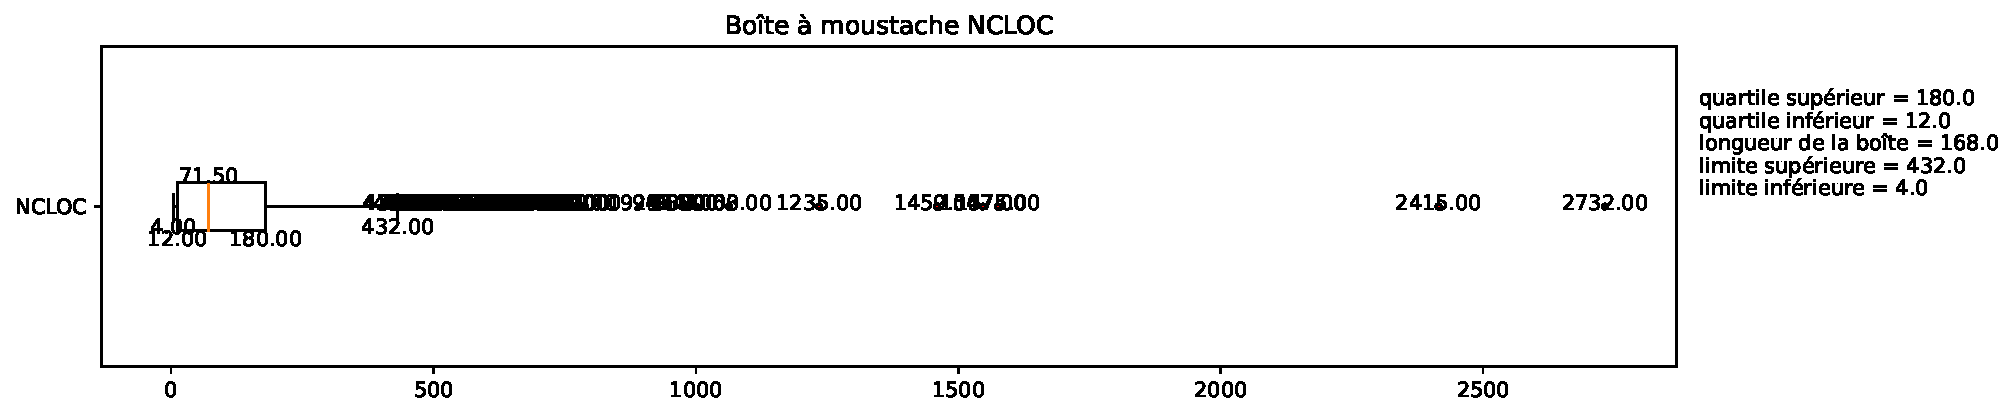
\includegraphics[scale=0.5]{assets/moustache_NCLOC}
    \centering
    \end{figure}
       Ici aussi, la boîte n'est pas symétrique et les variables ne sont donc encore une fois pas normalement distribuées, de plus on observe un nombre encore plus élevé de valeurs extrêmes. 
     \newpage
    \section{DCP}
    \begin{figure}[h]
    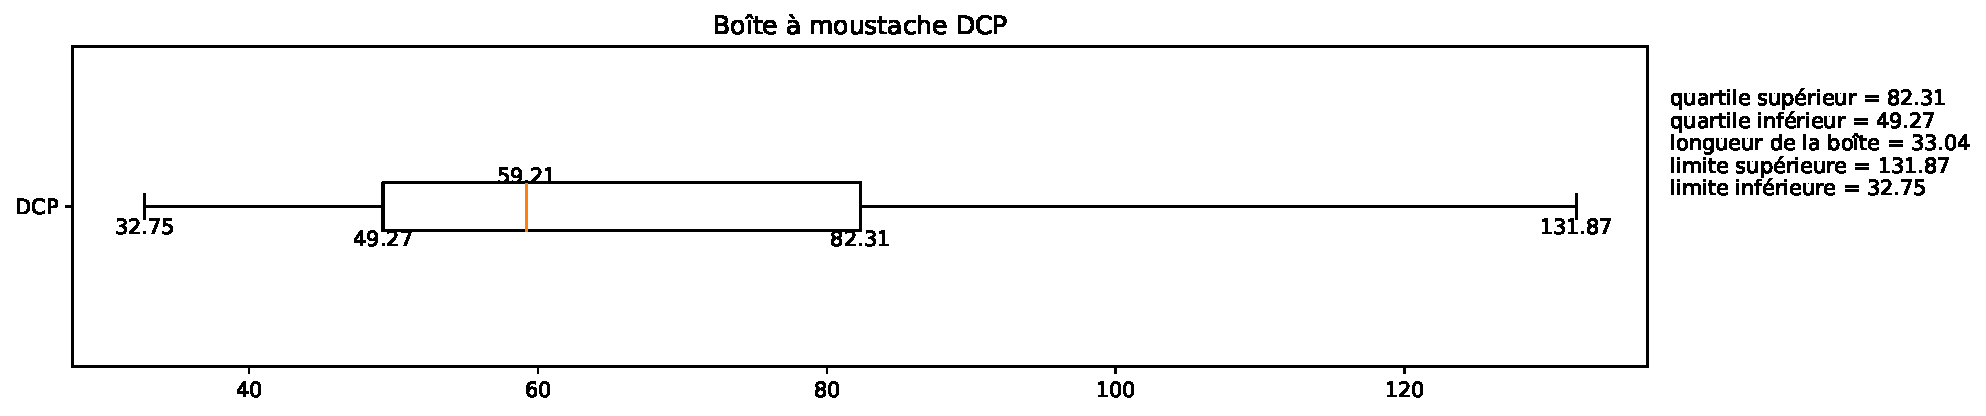
\includegraphics[scale=0.5]{assets/moustache_DCP}
    \centering
    \end{figure}
  Pour DCP, la boite bien que toujours asymétrique, les longueurs des moustaches sont sensiblement plus proches que dans les cas précédents et le placement de la médiane dans la boite est également plus centré, on note également l'absence de valeurs extrêmes, cela traduit donc une distribution des variables plus proche d'une distribution suivant la loi normale.
  
\chapter{Correlations}
    \section{NCLOC en fonction de NOCom}
    \begin{figure}[h]
    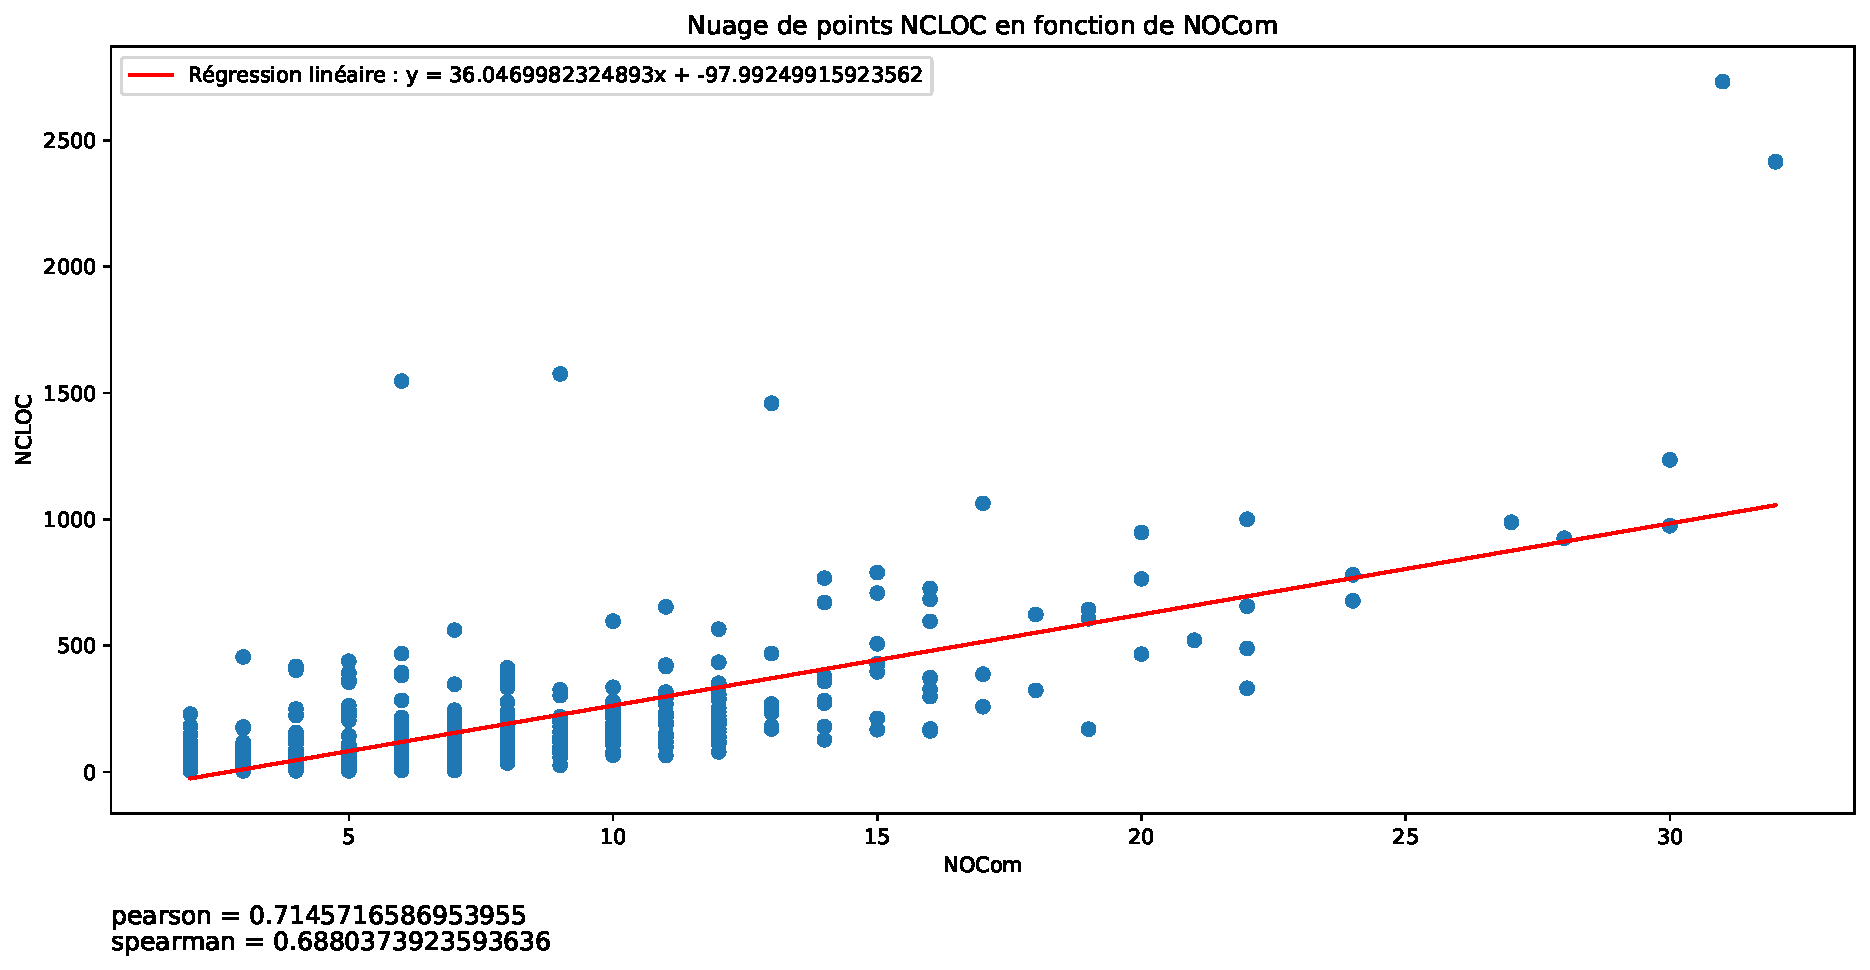
\includegraphics[scale=0.5]{assets/relation_NCLOC_NOCom}
    \centering
    \end{figure}
    On remarque que la plupart des points du graphique représentant NCLOC en fonction de NOCom semblent se répartir autour et en suivant une droite. Comme les variables ne sont pas normalement distribuées (cf la partie précédente), on utilise le coefficient de corrélation de Spearman et on trouve 0.688 ce qui témoigne d'une certaine relation relativement linéaire entre ces deux métriques puisque cette valeur est plus proche de 1 que de 0. On trouve alors en effectuant la régression linéaire l'équation suivante y = 36,05x - 97,99 décrivant cette relation.
     \newpage
    \section{DCP en fonction de NOCom}
 
    \begin{figure}[h]
    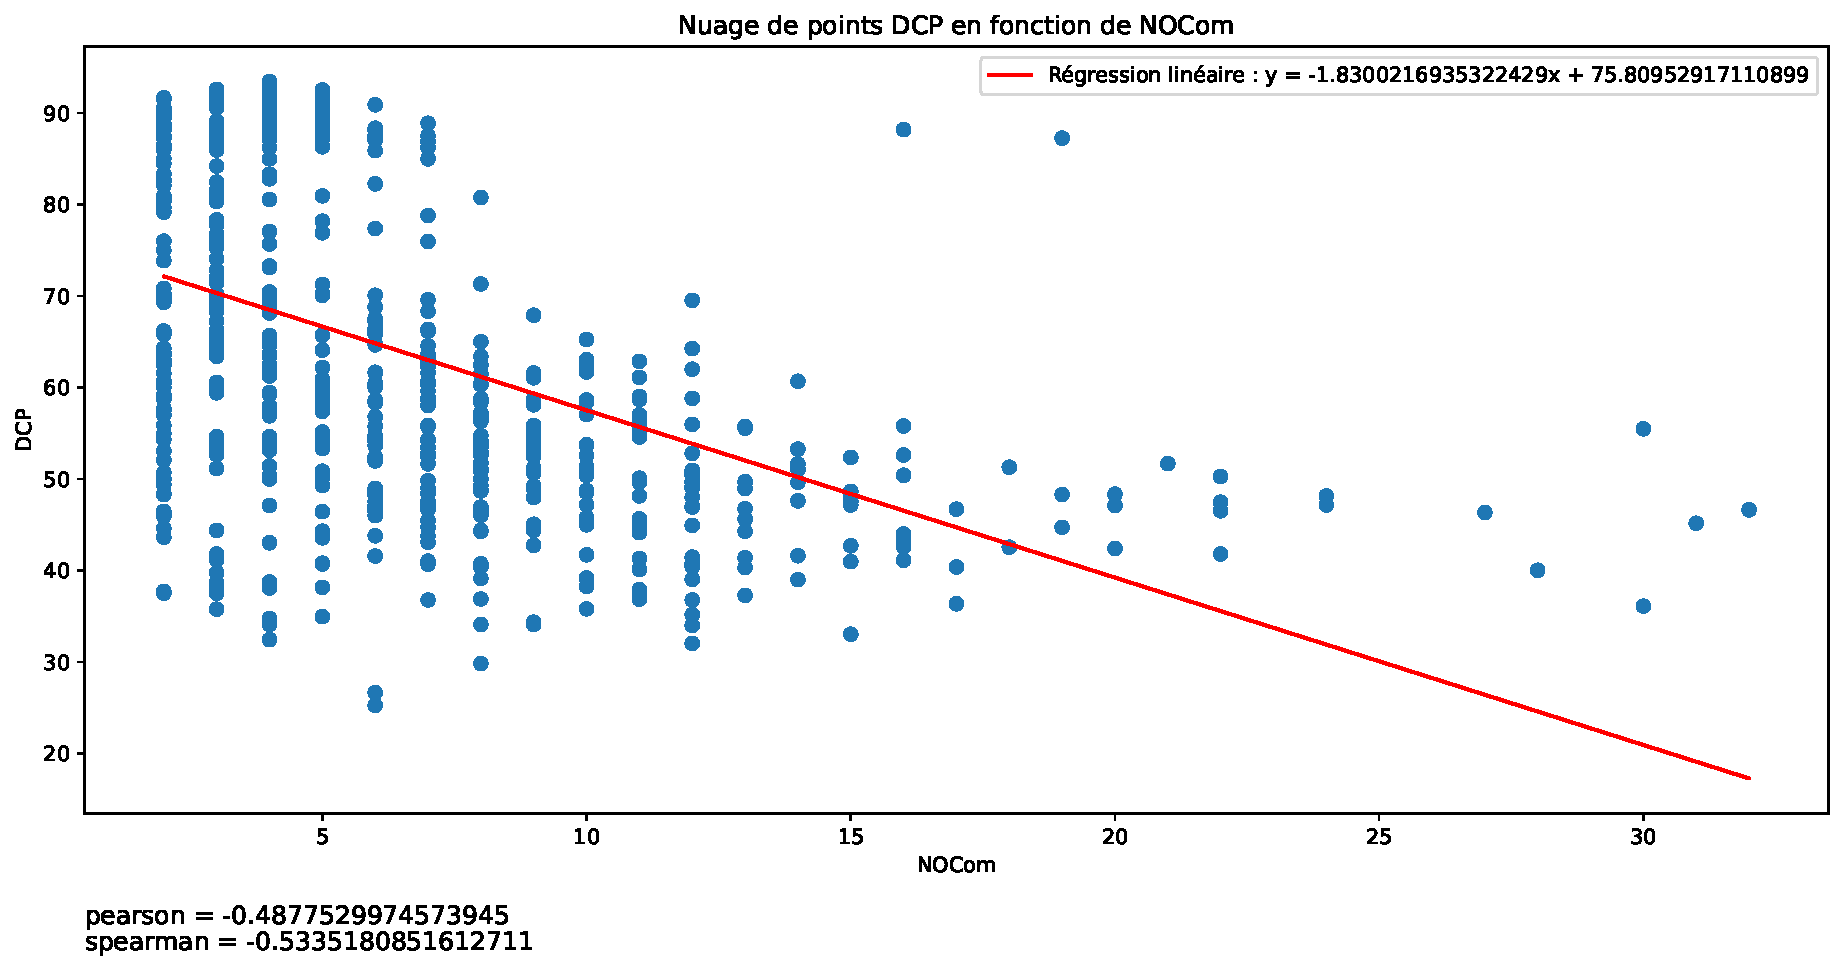
\includegraphics[scale=0.5]{assets/relation_DCP_NOCom}
    \centering
    \end{figure}

Ici, les points ne semblent pas vraiment suivre une même droite, cette observation est confirmée par la valeur de -0,53 du coefficient de Spearman qui bien que légèrement plus proche de -1 que de 0 ne constitue pas une valeur témoignant d'une relation très proche de la linéarité entre les deux métriques. Si on essaye toutefois d'obtenir une régression linéaire entre ces deux variables, on trouve l'équation y = -1,830x + 75,80.
    
\chapter{Quasi expérience}

\section{Choix d'étude}
Nous voulons évaluer l'impact du nombre de commits sur la qualité des commentaires d'une classe, cependant, il nous est impossible de faire varier directement le nombre de commits puisque celui-ci dépend de l'avancement en temps réel du développement des différents projets logiciels. C'est pourquoi nous allons faire une quasi-expérience.


\section{Hypothèse}


Notre hypothèse est la suivante : << les classes qui ont été modifiées plus de 10 fois sont mieux commentées que celles qui ont été modifiées moins de 10 fois >>.


\section{Définition et étude des variables}


La variable d’état sera le nombre de commits d'une classe puisque c'est un bon indicateur du nombre de fois que celle-ci a été modifiée, c'est ce paramètre qui en variant devra affecter le résultat de notre expérience.


La variable dépendante sera la densité de commentaire d'une classe, car cela permet de mesurer la quantité de commentaires au sein d'une classe relativement à son nombre de lignes de codes et donc d'estimer la qualité de l'état de commentaire de la dite classe.




Pour l'étude, nous effectuerons donc la quasi-expérience sur différents logiciels pour lesquels nous avons accès au dépôt git et nous sépareront les sujets en deux groupes, les classes ayant été modifiées moins de 10 fois et celles plus que 10 fois. Ensuite, pour chacun de ces groupes, nous évaluerons la qualité des commentaires avec la métrique DCP.

\section{Interprétation et généralisation des résultats}
Pour les deux groupes définis précédemment, nous pourront alors calculer par exemple la médiane de la valeur de DCP. Ensuite, en comparant les deux médianes, on pourra déterminer si oui ou non l'hypothèse est vérifiée et s'il existe donc bien une relation entre les deux variables choisies.

\section{Discussion des menaces à la validité}
\subsection{Validité de construction}
Les variables choisies permettent bien de modéliser l'hypothèse.
\subsection{Validité interne}
Nous ne pouvons pas être certains que le nombre de commits a réellement un impact sur la densité de commentaire puisqu'un commit signifie simplement que le fichier a été modifié. Par exemple, si une ligne vide a été ajoutée ou si le nombre de ligne de code reste le même entre deux commits, mais que du code a été modifié, la densité de commentaire restera identique.
\subsection{Validité externe}
En fonction de la complexité de la tâche réalisée par les logiciels ou du langage dans lequel ils sont écrits, il se peut qu'une faible ou une grande quantité de commentaire soit nécessaire afin d'avoir un bon niveau de compréhension et de maintenabilité de la classe et donc suivant les cas sélectionnés pour l'étude, il se peut qu'il ne soit pas possible de généralisé la conclusion à l'ensemble des projets logiciels et/ou des langages de programmation.
\subsection{Validité de conclusion}
Comme décrit lors de la section sur la validité interne, nous ne pouvons être certains que le nombre de commits est bien responsable de la modification de la densité de commentaire d'une classe. Il sera donc possible de tirer des conclusions fausses de cette étude.
\end{document}